\chapter{Experiments}\label{experiments}

This study aims to investigate how different semantic search techniques, input patterns, and models can be used to predict political party stances.

A series of experiments is conducted to compare the effectiveness of six semantic search techniques (plus two variations), examine the impact of five different input patterns, and explore the effectiveness of two language models.

 
\section{Semantic Search}

The various methods for semantic search presented in chapter \ref{semantic_search} are applied to all sentences in the 2021 party manifestos. These sentences are shuffled, since this significantly affects the outcomes according to \citet{li2020bertflow}. The semantic search models are then applied to this shuffled dataset. There are a total of eight different methods used:

\begin{itemize}
    \item \textbf{BM25}: use the BM25+ algorithm as described in \citet{lv2011lower}, it is implemented in the python package \textit{rank\_bm25} by \citet{rank_bm25}. This is the only algorithm from the list that has nothing to do with BERT \citep{devlin2018bert}. It was chosen as a baseline to compare the more sophisticated methods to.
    \item \textbf{SBERT}: the sentence embeddings are obtained by using the pre-trained ``paraphrase-multilingual-mpnet-base-v2'' model \citep{reimers-2020-multilingual-sentence-bert} from the python package \textit{sbert} by \citet{reimers2019sbert}. ``Paraphrase-multilingual-mpnet-base-v2'' is chosen since it is the highest-performing multilingual model according to \citet{reimers_2022}.
    \item \textbf{BERT-Flow}: two BERT-Flow models get trained following \citet{li2020bertflow}, one uses ``bert-base-german-cased'' \citep{german_bert} to obtain the base embeddings (from now on called ``BERT-Flow'') and the other uses the SBERT model ``paraphrase-multilingual-mpnet-base-v2'' \citep{reimers-2020-multilingual-sentence-bert} (from now on called ``SBERT-BERT-Flow''). The code used has been altered from \citet{pytorch-bertflow}.
    \item \textbf{Whitening}: the Whitening transformation from \citet{huang2021whiteningbert} is also applied to two models. ``Bert-base-german-cased'' \citep{german_bert} (from now on called ``Whitening'') and ``paraphrase-multilingual-mpnet-base-v2'' \citep{reimers-2020-multilingual-sentence-bert} (from now on called ``SBERT-Whitening'').
    \item \textbf{SBERT-WK}: the code from ``SBERT-WK-Sentence-Embeddings'' \citep{sbert-wk} (Github repository following the paper from \citet{wang2020sbertwk}) is used to train a model that uses ``bert-base-german-cased'' \citep{german_bert} as its base model.
    \item \textbf{IS-BERT}: using ``bert-base-german-cased'' \citep{german_bert} as the base model, a model as described by \citet{zhang2020isbert} is trained. The code is from the ``IS-BERT'' repository \citep{isbert}.
\end{itemize}

These eight methods are applied to the queries to get the five most semantically similar sentences from each of the parties manifestos. For all methods except BM-25, that means computing the dot score between the embeddings of the query and all sentences in the manifesto and choosing the five sentences with the highest dot score.

\section{Input Pattern Design} \label{exp_patterns}

The input that gets fed into the model can be built from three ``building blocks'':

\begin{itemize}
    \item \textcolor{violet}{\textbf{Party}}: the name of the party the model should predict agreement for: \textit{spd}, \textit{cdu} (stands for both CDU and CSU), \textit{grüne}, \textit{fdp}, \textit{afd} or \textit{linke}.
    \item \textcolor{olive}{\textbf{Query}}: the user-generated input sentence (for example: ``BAföG für alle Studierenden'').
    \item \textcolor{teal}{\textbf{Context}}: 
    \begin{itemize}
        \item Up to five sentences from the party manifesto that relate to the user query which are found using the different semantic search techniques.
        \item They are added as a list with square brackets [...] to indicate the beginning and the end.
        \item If the input is longer than 512 tokens (the maximum input length for the models) for a certain semantic search method, only four (or, if necessary, three) sentences are used as context. This is the case for BERT-Flow (four sentences), SBERT-BERT-Flow (three sentences), and IS-BERT (three sentences).
    \end{itemize}
\end{itemize}

From these building blocks, five different patterns (plus two variations) are built.\\

\textbf{Baseline}:

\begin{center}
    \textcolor{violet}{<party>}: \textcolor{olive}{<query>}
\end{center}
for example: \textcolor{violet}{linke}: \textcolor{olive}{‘BAföG für alle Studierenden’} 

This is the same input that \citet{witte_2022} use to train their model. The input doesn't contain any context and therefore serves as the baseline. By comparing the other input patterns with it, it is possible to determine if adding context improves the performance.\\

\textbf{No additional text} (pattern 1-1):

\begin{center}
    \textcolor{violet}{<party>}: \textcolor{teal}{<context>}, \textcolor{olive}{<query>}
\end{center}
for example: \textcolor{violet}{linke}: \textcolor{teal}{['Wir setzen uns für ein rückzahlungsfreies, elternunabhängiges und bedarfsgerechtes BAföG ein, das alle erreicht, die es brauchen.', 'Das führt zu Stress bei Studierenden und Beschäftigten.', 'Ebenso muss die Kopplung des BAföG an Leistungsüberprüfungen abgeschafft werden.', 'Nur noch 11 Prozent der Studierenden erhalten überhaupt BAföG, nur 8 Prozent den Höchstsatz.', 'Das BAföG muss an die Lebenswirklichkeit angepasst werden und die Ausbildung umfassend finanzieren.']}, \textcolor{olive}{‘BAföG für alle Studierenden’}

a variation of this is pattern 1-2:
\begin{center}
    \textcolor{violet}{<party>}: \textcolor{olive}{<query>}, \textcolor{teal}{<context>}
\end{center}

Simply concatenating the different building blocks results in these two patterns. But the model is not given any more information on what exactly it is that it receives. It is also of interest if the order of the building blocks matters.\\

\textbf{Minimal text} (pattern 2-1):

\begin{center}
    \textcolor{violet}{<party>}: Satz: \textcolor{olive}{<query>}, Kontext: \textcolor{teal}{<context>}
\end{center}
for example: \textcolor{violet}{linke}: Satz: \textcolor{olive}{‘BAföG für alle Studierenden’}, Kontext: \textcolor{teal}{['Wir setzen uns für ein rückzahlungsfreies, elternunabhängiges und bedarfsgerechtes BAföG ein, das alle erreicht, die es brauchen.', ..., 'Das BAföG muss an die Lebenswirklichkeit angepasst werden und die Ausbildung umfassend finanzieren.']}

and as a variation pattern 2-2:
\begin{center}
    \textcolor{violet}{<party>}: Kontext: \textcolor{teal}{<context>}, Satz: \textcolor{olive}{<query>}
\end{center}

Here, the model gets added information. It now knows that the query is the ``Satz'' (sentence) and the context is the ``Kontext'' (context). Does this improve the performance, or is this extra information not needed?\\

\textbf{Human-speech-like} (pattern 3):

\begin{center}
    Passt \textcolor{olive}{<query>} zur \textcolor{violet}{<party>} und \textcolor{teal}{<context>}?
\end{center}

for example: Passt \textcolor{olive}{‘BAföG für alle Studierenden’} zur \textcolor{violet}{linke} und \textcolor{teal}{['Wir setzen uns für ein rückzahlungsfreies, elternunabhängiges und bedarfsgerechtes BAföG ein, das alle erreicht, die es brauchen.', ..., 'Das BAföG muss an die Lebenswirklichkeit angepasst werden und die Ausbildung umfassend finanzieren.']}? \\

\textbf{Human-speech-like} (pattern 4):

\begin{center}
    \textcolor{violet}{<party>} sagt: \textcolor{teal}{<context>}, passt \textcolor{olive}{<query>} dazu?
\end{center}
for example: \textcolor{violet}{linke} sagt: \textcolor{teal}{['Wir setzen uns für ein rückzahlungsfreies, elternunabhängiges und bedarfsgerechtes BAföG ein, das alle erreicht, die es brauchen.', ..., 'Das BAföG muss an die Lebenswirklichkeit angepasst werden und die Ausbildung umfassend finanzieren.']}, passt \textcolor{olive}{‘BAföG für alle Studierenden’} dazu? \\

Patterns 3 and 4 are similar to how a human would ask a question. This is the style of input a language model like ChatGPT \citep{chatgpt} would like to receive. It is of interest to see if this also works for the models used here. \\

That means that, together with the eight different semantic search methods, there are now (8*6)+1 = 49 different inputs.

\section{Models}

The various inputs are fed into two different models. The two models that are used are:

\begin{itemize}
    \item \textbf{ELECTRA}: ``electra-base-german-uncased'' \citep{german_electra} is used and fine-tuned for 13 epochs with a learning rate of 2.21e-5 (since those were the optimal hyper-parameters in the experiments of \citet{witte_2022})
    \item \textbf{BERT}: ``bert-base-german-cased'' \citep{german_bert} is used and trained for 11 epochs with a learning rate of 1.95e-5 (hyper-parameters also taken from \citet{witte_2022})
\end{itemize}

The decision to use the ELECTRA and BERT models was based on a number of factors. First of all, these models were selected because \citet{witte_2022}, on which this project is based, tested them. Second, the models' size had to be taken into account in order for them to fit within the computing resources available and still provide good performance. Both ELECTRA and BERT were found to be sufficiently compact for the needs of the project and to deliver results that were competitive. Both models are also well-known in the NLP community, and a substantial body of research backs their efficacy. These factors made the ELECTRA and BERT models an ideal choice for the project's needs.

\begin{figure}[h!]
\centering
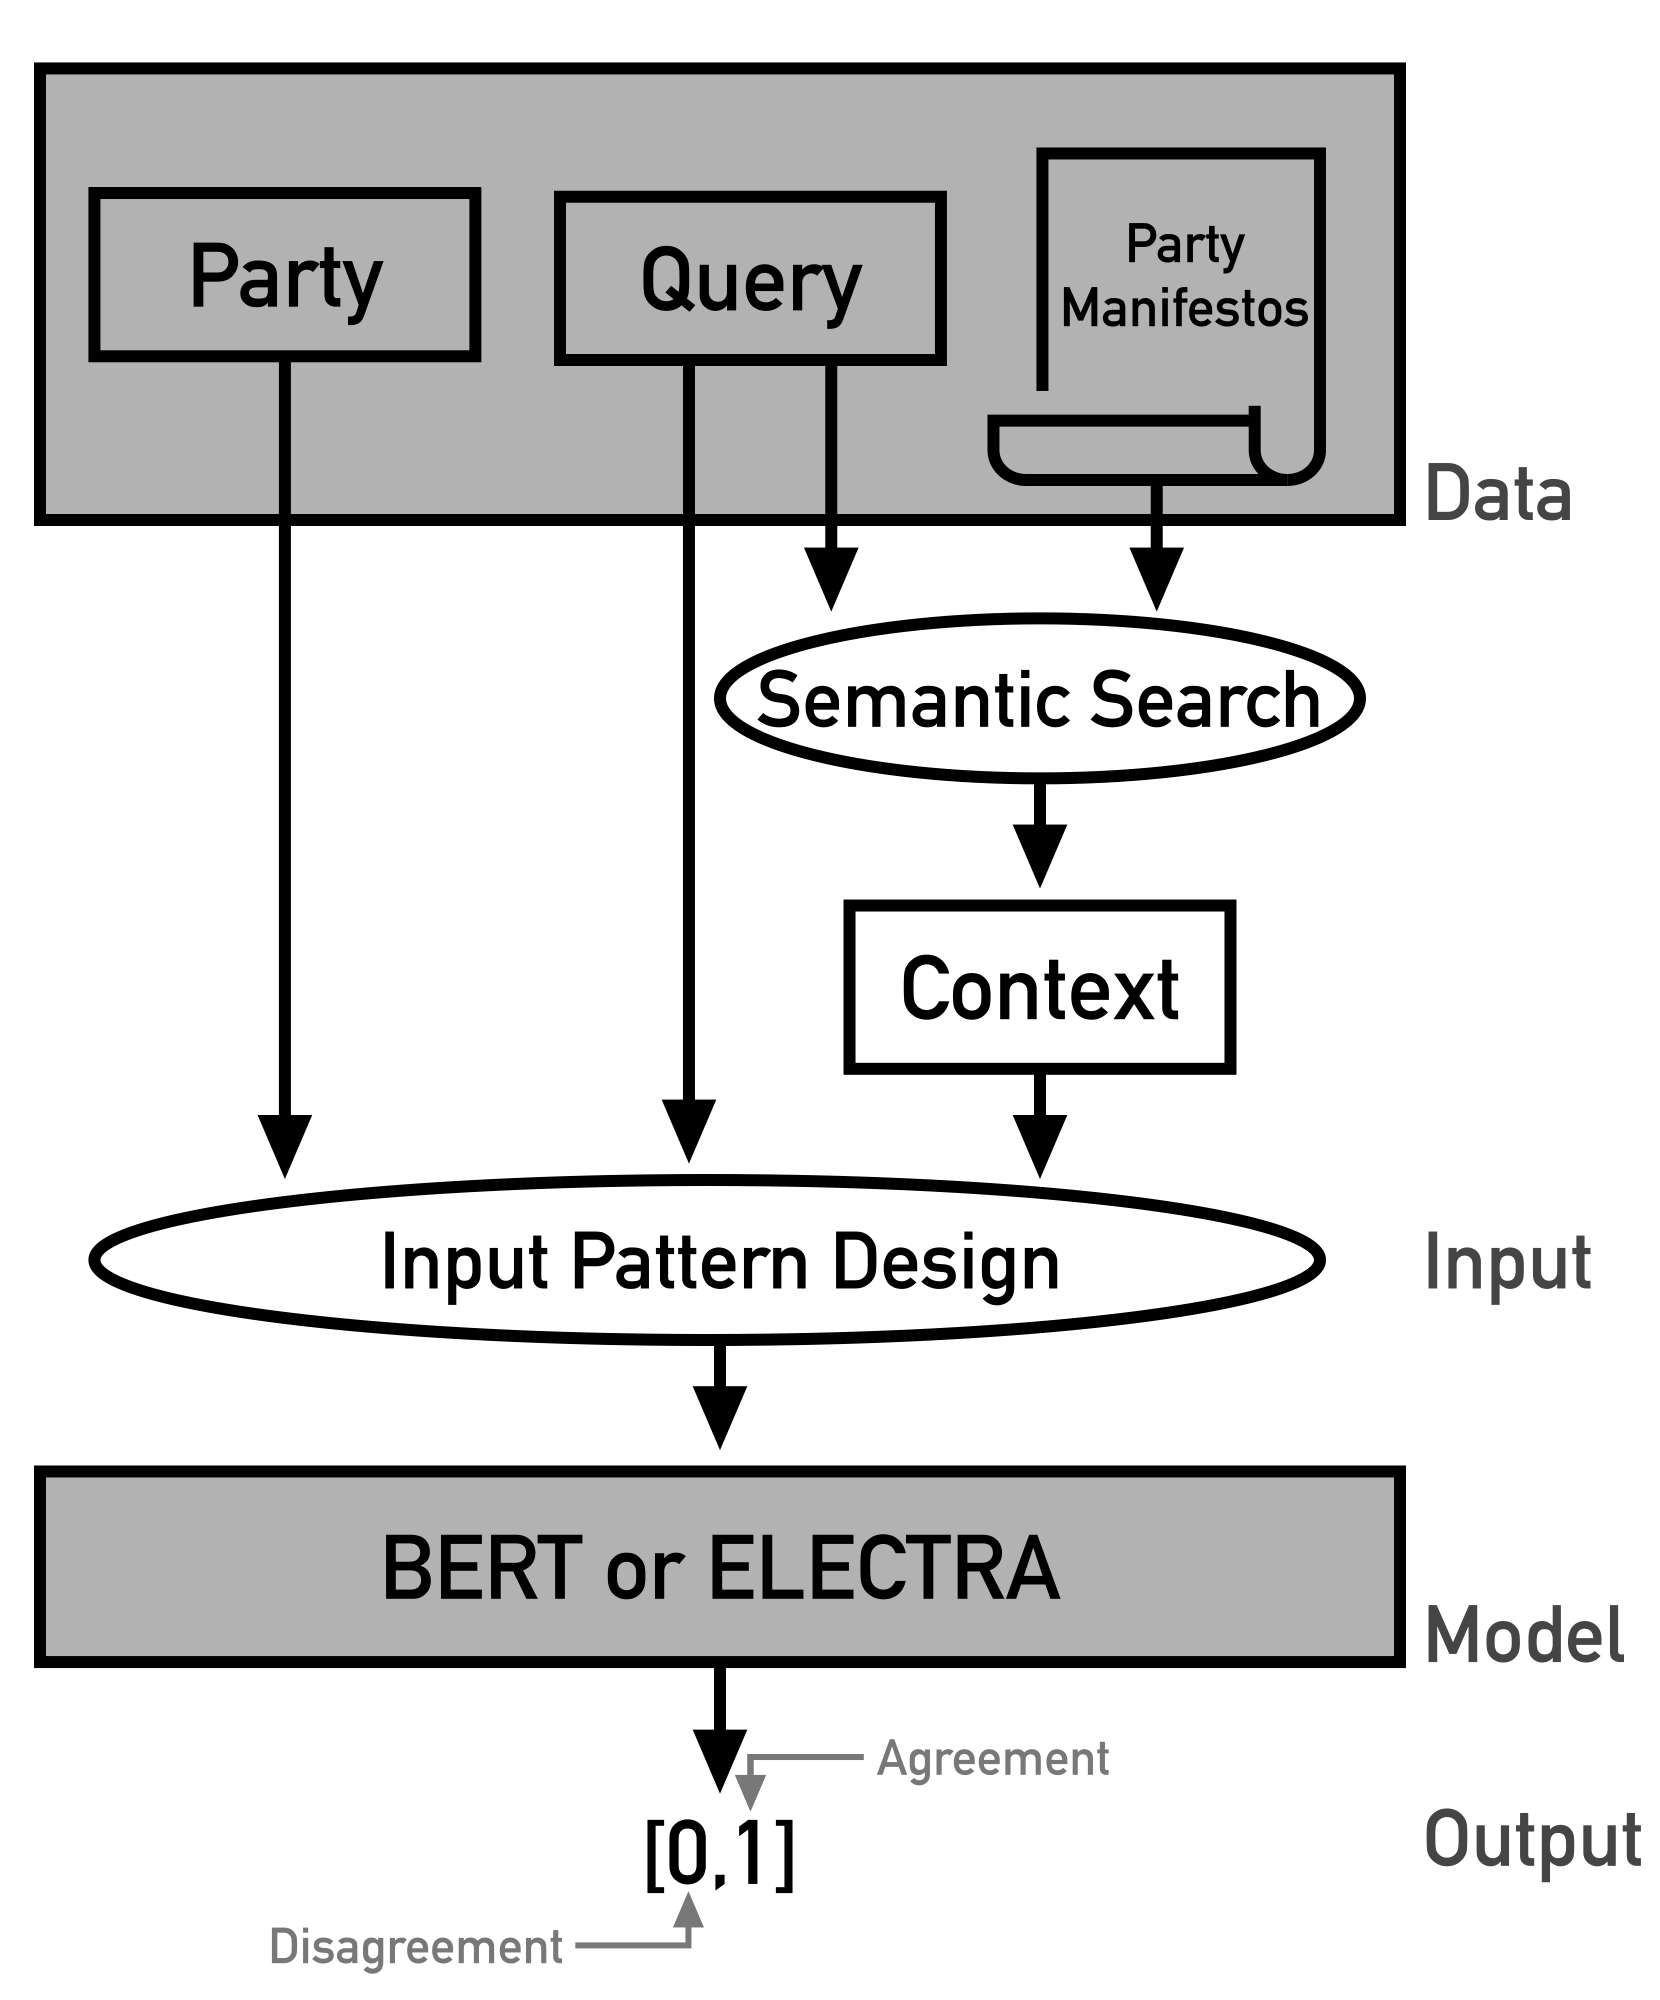
\includegraphics[width = 0.6\linewidth]{figures/Experiments1.png}
\caption{An illustration of the experiments' approach.}
\label{fig:experiments1}
\end{figure}

Figure \ref{fig:experiments1} illustrates how the experiment is set up. Having two models means that there are now 49*2= 98 different predictions for every user query. The goal is to find the combination that works best and see if there are any semantic search techniques or input pattern designs that work better than others. It is also of interest if adding sentences from the manifestos as context even had any effect on the performance of the models.

\section{Evaluation}

To evaluate the performance, about 30\% of the data is held back as testing data and is not used for training. By calculating the accuracy and F1 score using the test data, the models' performance is assessed. 

The percentage of instances that are correctly classified out of all instances is measured by the accuracy metric. It is given by the formula:

\begin{equation}
\text{Accuracy} = \frac{\text{Number of Correctly Classified Instances}}{\text{Total Number of Instances}}
\end{equation}

For instance, the model's accuracy is 90\% if it correctly predicts 90 out of 100 party stances. Since accuracy is simple to comprehend and interpret, it is frequently used to evaluate model performance. However, it can be misleading in some cases, especially when the classes are imbalanced.

F1 score is a better metric than accuracy when the classes are imbalanced, because it takes both precision and recall into account. Precision measures the percentage of true agreements out of all predicted agreements, while recall measures the percentage of true agreements out of all actual agreements. F1 score is given by the formula:

\begin{equation}
\text{F1 Score} = 2 \times \frac{\text{Precision} \times \text{Recall}}{\text{Precision} + \text{Recall}}
\end{equation}
F1 is also useful when the cost of false agreement and false disagreement predictions are different. For example a false disagreement (a party not agreeing being classified as agreeing to a stance) could be more costly than a false agreement (an agreeing party being classified as disagreeing). However, it appears that this is not the case in this context. The classes are also not imbalanced, the amount of agreement and disagreement is approximately the same both for the training and the testing data. For this reason, the F1 score results are included in the appendix \ref{f1}.

\section{Further Experiments} \label{exp_further}

As of now, the context consists solely of statements taken directly from the party manifestos. Another option is to condense these five (or, in some cases, four or three sentences) into a single sentence that, ideally, includes all of the relevant information. As the summarized context should be much less complex and contains less unnecessary noise, this might improve the performance of the model. Additionally, it is shorter, which might make it simpler for the model to ``remember''.

IGEL \citep{igel}, which stands for \textbf{I}nstruction-tuned \textbf{Ge}rman large \textbf{L}anguage Model, is a family of LLMs developed specifically for the German language. The BigScience BLOOM architecture \citep{bloom}, notably the BLOOM-CLP German version by \citet{bloom-german}, is the foundation of IGEL. A dataset of instructions that have been automatically translated from English to German is used to train the model. Hallucination, toxicity, and stereotypes—common flaws in language models—are some of IGEL's acknowledged drawbacks. It is utilized in this instance to obtain one sentence summaries.

In order to do this IGEL is given the command: ``Als eins Satz zusammenfassen: \textcolor{teal}{<context>}''. This roughly translates to ``Summarize in one sentence: \textcolor{teal}{<context>}'', but the number ``eins'' is used in place of the correct word ``ein''. This is done because testing revealed that doing so improved the model's comprehension of the fact that it only needed to produce one sentence.

However, this still frequently fails, as evidenced by the summary results for the example context:
\textcolor{teal}{[’Wir setzen uns für ein rückzahlungsfreies, elternunabhängiges und bedarfsgerechtes BAföG ein, das alle erreicht, die es brauchen.’, ’Das führt zu Stress bei Studierenden und Beschäftigten.’, ’Ebenso muss die Kopplung des BAföG an Leistungsüberprüfungen abgeschafft werden.’, ’Nur noch 11 Prozent der Studierenden erhalten überhaupt BAföG, nur 8 Prozent den Höchstsatz.’, ’Das BAföG muss an die Lebenswirklichkeit angepasst werden und die Ausbildung umfassend finanzieren.’]}.

This context is summarized by IGEL as four rather than one sentence:
\textcolor{teal}{``Wir fordern eine elternunabhängige, bedarfsgerechte und rückzahlungsfreie Ausbildung, die alle erreicht. Das führt zu Stress bei Studierenden und Beschäftigten, und der Studienerfolg ist unzureichend. Daher fordern wir, die Verknüpfung des BAföG mit Leistungsüberprüfungen abzuschaffen. Wir fordern auch, dass die Ausbildung mit dem realen Leben Schritt hält und die Ausbildung umfassend finanziert wird.''}

The structure of the experiments, including the summary experiment, is depicted in Figure \ref{fig:experiments2}. Because IS-BERT has proven to be the most effective semantic search technique (see Chapter \ref{results}), only contexts obtained using this method will be used in the experiment. Once the summary is generated, the resulting summary will be used as the context for the model, employing the different input patterns described in Chapter \ref{exp_patterns}. Only ELECTRA will be used out of the two models because it has been found to produce the best results (again see Chapter \ref{results}). The results will be discussed by examining the accuracy, with the F1 score results located in the appendix, just like for the other models.

\begin{figure}[h!]
\centering
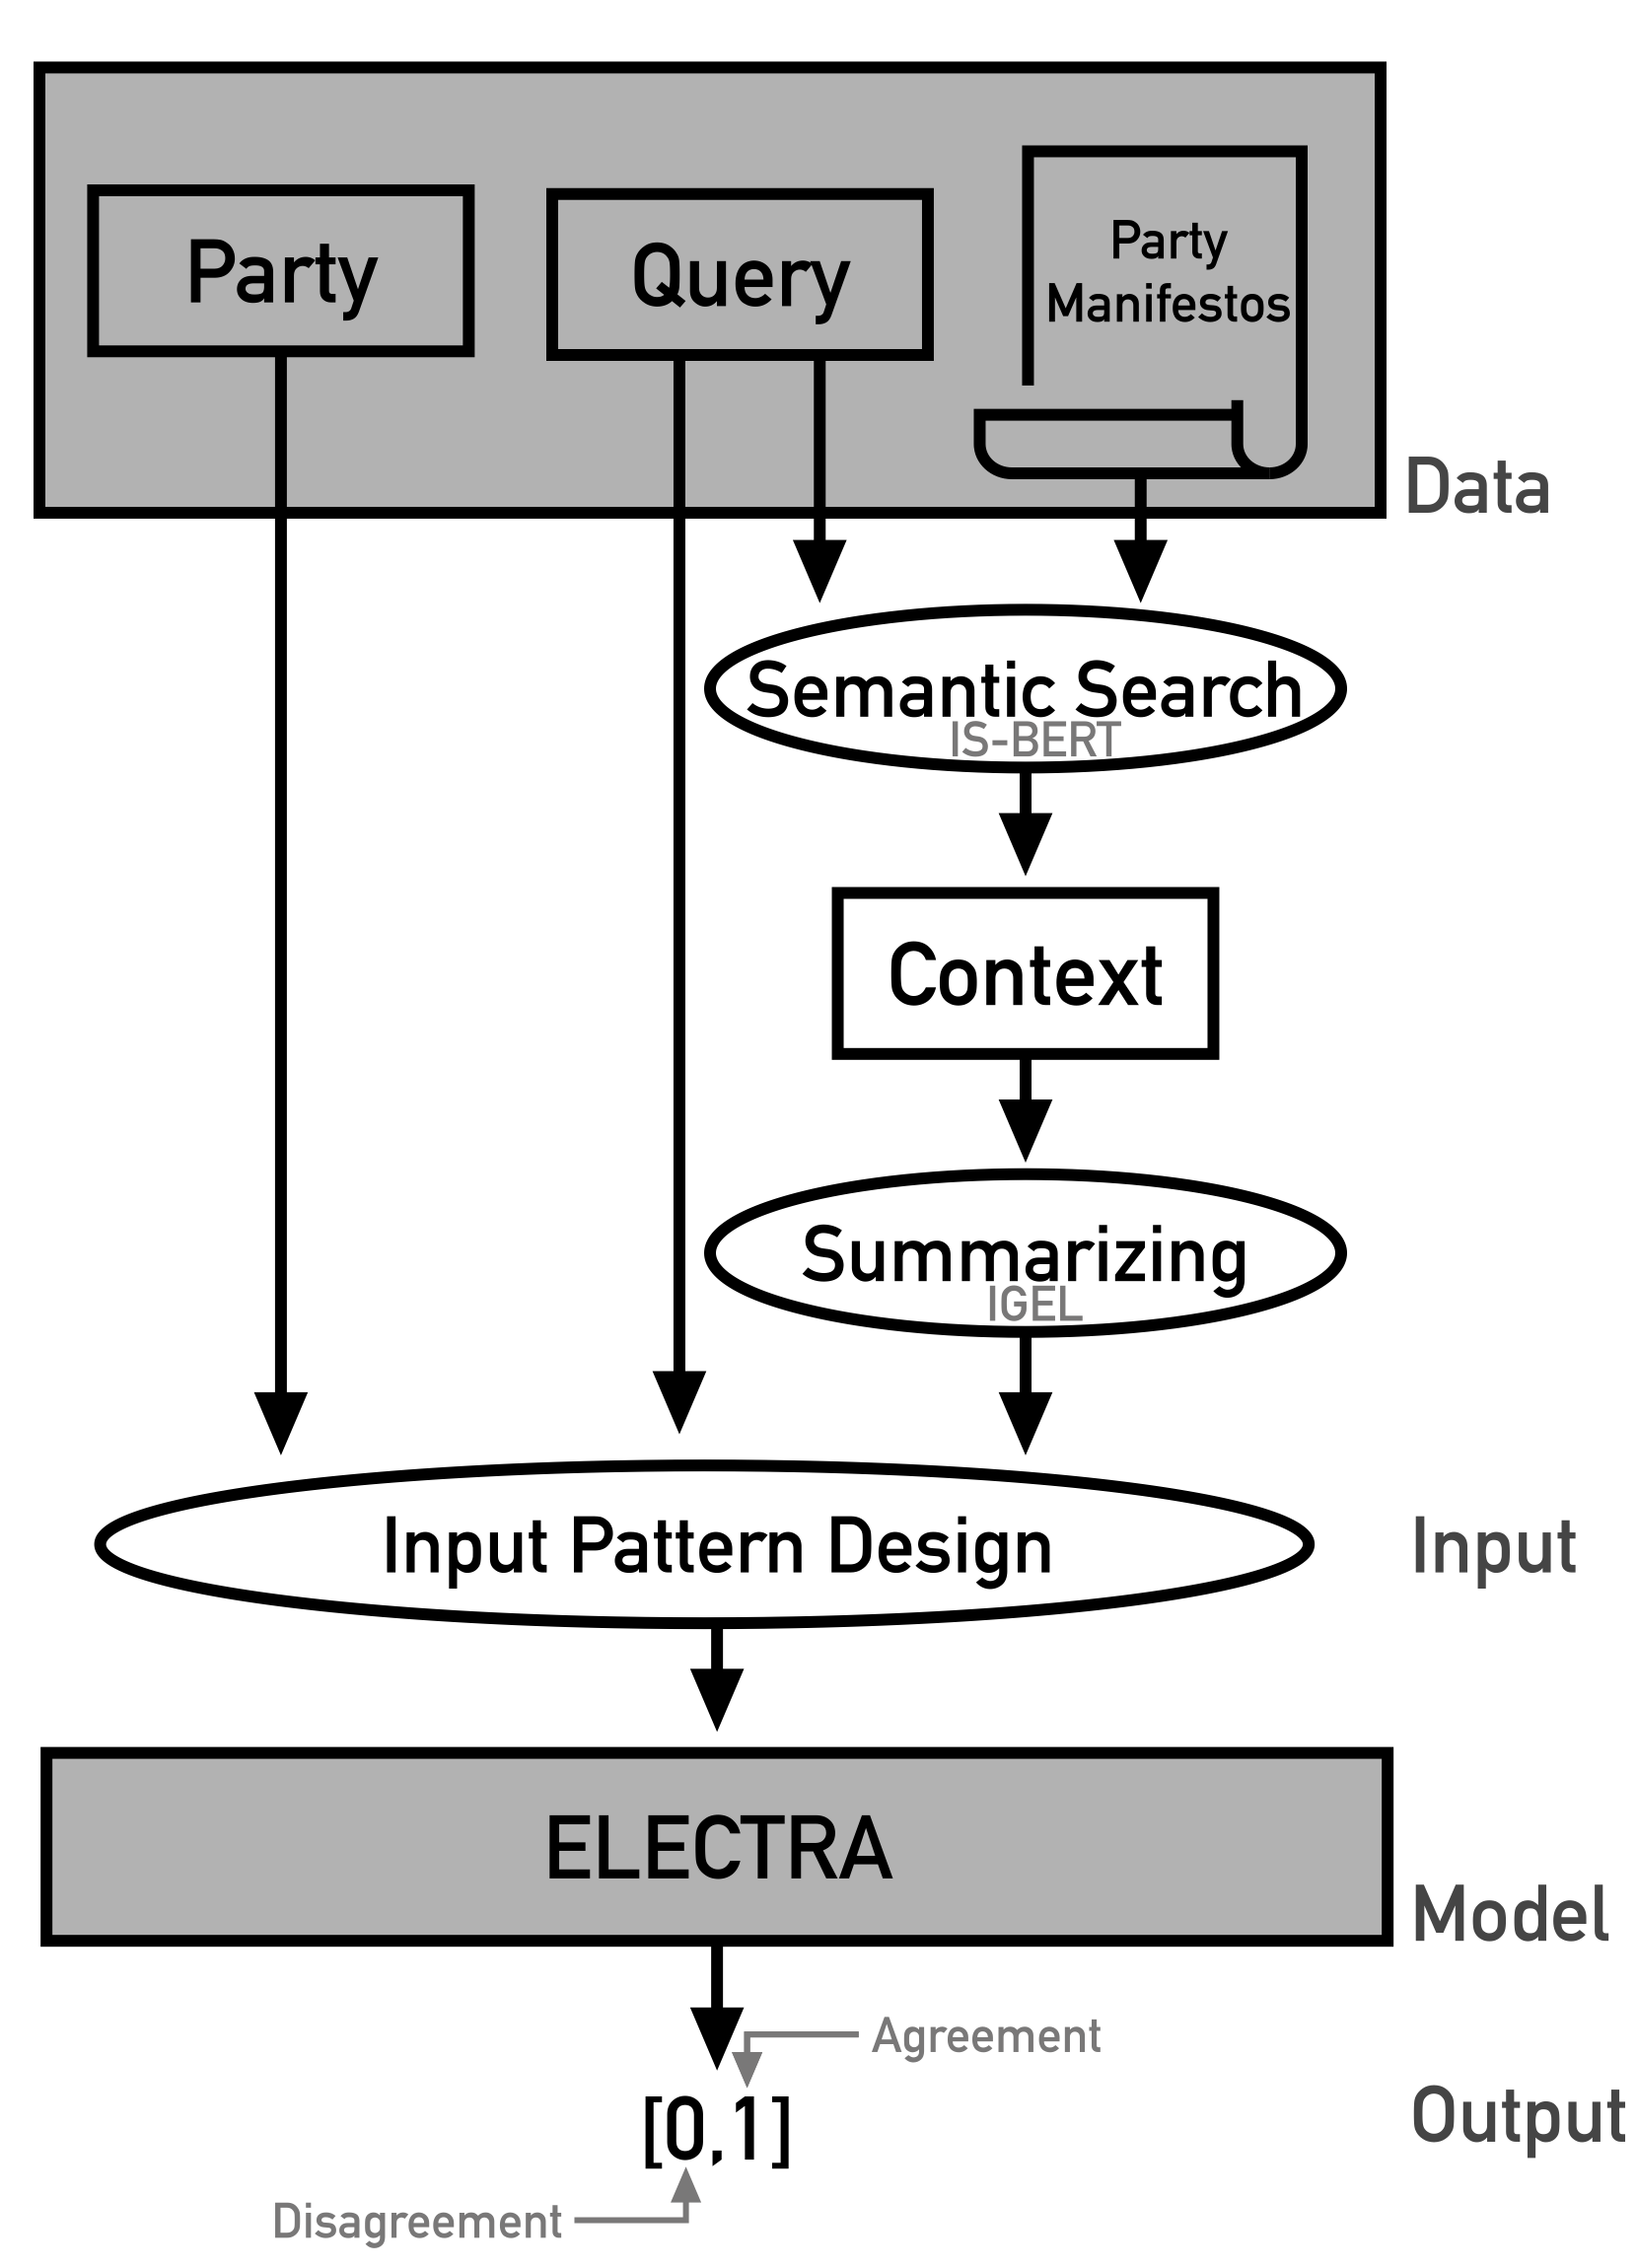
\includegraphics[width = 0.6\linewidth]{figures/Experiments2.png}
\caption{An illustration of the experiments' approach with summarization.}
\label{fig:experiments2}
\end{figure}
